\documentclass[10pt,a4paper,twocolumn]{article}
\newcommand\tab[1][0.5cm]{\hspace*{#1}}
\title{%
		Model-free Reinforcement Learning: Q-Learning \\
	\large Course assignment: Machine Learning \\
			University of Piraeus, Demokritos}
\author{
	Sarafidis, Tasos\\
	\texttt{sar.tasos@gmail.com}
	\and
	Papadopoulos, Vasileios\\
	\texttt{vassilispapadop@gmail.com}
}

\usepackage[utf8]{inputenc}
\usepackage[T1]{fontenc}
\usepackage{amsmath}
\usepackage{amsfonts}
\usepackage{amssymb}
\usepackage{graphicx}
\usepackage{amsmath}
\usepackage{graphicx}
\usepackage{hyperref}
\graphicspath{ {./images/} }


\begin{document}
	\maketitle
	
	\section{Reinforcement Learning}
	Reinforcement Learning is an area of Machine Learning, where the main purpose is to find a way for an agent to learn a policy by interacting with its environment. An agent lives within an environment and interacts with it by examining the state in which it is in, for every time step. After examining its state, the agent chooses an action and the environment returns the corresponding reward, as well as the agent’s new state. The agent’s goal is to find the actions that return the most reward by trying them, without knowing which actions to choose beforehand. This means, the agent must discover the best action that will allow it to learn the optimal policy towards achieving its goals.
	
	In Reinforcement Learning problems, the agent is always in interaction with the environment. In every time step t, the agent receives a state of the environment, st, and chooses an action, at. In the next time step, the agent gets a reward, $r_{t+1}$, from the environment and moves to the next state, $s_{t+1}$. In every step, the agent assigns a state to an action thus forming the agent’s policy, $\pi_{t}$.
	
	Problems in the area of Reinforcement Learning are usually modeled as Markov Decision Processes (MDPs). A MDP is a time-discrete stochastic control process, where agents’ actions affect immediate and future rewards, as well as next states. A Markov Decision Process can be described by a tuple {S,A,R,T}, where:
	
	\begin{itemize}
		\item S is the set of all possible states. 
		\item A is the set of actions.
		\item R(s) is the reward function, which returns a numerical value as a result of an agent’s action.
		\item $T(s,\alpha,s')$ is the state transition function, which given a state s and an action $\alpha$ returns the next state s'.
	\end{itemize}
	
	\section{Multi-Agent Systems}
	A Multi-Agent System is a set of agents who interact with each other and have a common or contradictory goal. In multi-agent systems, each agent is a part of the other agents’ environment, meaning that as an agent learns and looks for the best policy, the results of its actions depend, not only on its state, but also on the other agents’ actions. Agents either cooperate with each other to achieve a common goal, or come into conflict with each other in order to succeed their personal goals.
	
	The Markov Decision Process that was described in section 1, can be also expanded on multi-agent systems and can be denoted by a tuple (Ag, S,A,R,T):
	
	\begin{itemize}
		\item Ag is set of agents. 
		\item S is set of states.
		\item A is set of possible actions.
		\item R is the reward function.
		\item T is the transition function.
	\end{itemize}


	\section{Q-Learning}
	Q-Learning is an off-policy reinforcement learning algorithm that allows an agent to choose the best action in a given state. When the agent is in a state and performs an action, the environment returns the reward and the agent’s next state. Then, the agent estimates the value of the new state. Each time an agent chooses an action and learns about its new state, the overall value of the executed action in the corresponding state is updated by the \textit{update rule}:
	
	\begin{equation}
		\begin{aligned}
			Q(s,a) = Q(s,a) + a[R(s,a) + \gamma \\
			\max{Q(s',a') }- Q(s,a)]
		\end{aligned}
	\end{equation}
	
	where $0 < \alpha \le 1$ is the learning rate, $0 \le \gamma \le 1$ is the discount rate which determines the values of future rewards for a given time, and s' is the agent’s next state after performing its action. The overall value is called Q-value and is stored in the Q-table, which is later being used by the agent to read the stored values.
	
	There are two ways for an agent to choose its action in each state. Firstly, the agent chooses randomly its next action without looking up the Q-table. This method is called \textit{exploration}. The second way of choosing its action is called \textit{exploitation}. According to this, the agent looks up the Q-table to find out which action has the best Q-value and execute it.
	
	But, how does the agent decide whether to explore or exploit? This is done by using the $\epsilon - greedy$ algorithm. This algorithm states that with a probability of $0 \le \epsilon \le 1 $  an agent chooses to explore and with a probability of  the agent chooses to exploit the Q-table.


	\section{Problem Formulation}
	
	In our assignment we were faced with a symmetrical game of cooperation between two agents, the agent \textit{Row} and the agent \textit{Column}. Each agent interacts with the environment, which in return gives the agents their reward, based on the combination of both their actions (Table 1).
	


\begin{table}[h!]
	\centering
	\begin{tabular}{|c c c|} 
		\hline
		 & A & D  \\ [0.5ex] 
		\hline\hline
		A & $\alpha,\beta$  & $\beta,\alpha$  \\
		D & $\alpha,\beta$ & $\delta,\epsilon$  \\ [1ex] 
		\hline
	\end{tabular}
		\caption{Reward Matrix \label{overflow}}
	\end{table}

	According to Table 1, if both agents choose action A then agent \textit{Row} will get reward $\alpha$ and agent \textit{Column} will get reward $\beta$. Equally, if both agents choose action D, then \textit{Row} will get reward $\beta$ and \textit{Column} will get reward $\alpha$. On the other hand, if Row performs action A and Column chooses action D, then their rewards will be $\delta, \epsilon$ respectively. Finally, if Row decides to choose action D and Column action A, their respective rewards will be $\epsilon, \delta$. It must be noted that the agents do not have any knowledge about the other agent’s actions and their goal is to choose the action that maximizes their personal expected payoff.

	The purpose of our assignment is to develop a Q-Learning $\epsilon$-greedy algorithm which learns to play the game and satisfy the agents goals. To achieve that, after developing the algorithm, our two-agents system runs 20 rounds per episode, for a total of 100 episodes. In each round, agents choose their actions and the environment returns a reward to each one of them. At this point, the round is finished, the Q-values of each agent are computed and they are updated in the Q-table. After running 20 rounds, the episode ends and a new episode starts from the beginning resetting everything except for the Q-table. This process is repeated until 100 episodes are completed.
	
	\section{Implementation}
	
	In our implementation we used the programming language \textit{Python} and \textit{numpy}, \textit{pandas} and \textit{matplotlib} packages. To represent the problem, we make use of pandas \textit{DataFrame} object. We created the class \textit{Agent} to describe the contents of the entity \textit{agent}  in the context of MDP framework. In particular, we let the agent to choose its \textit{next-action}, discover environment states, update its q-table and store statistics. The function \textit{next-action} implements the \textit{$\epsilon-greedy$} strategy to explore different states it could encounter. Implementation is shown below.
	
	if np.random.random() < self.e-greedy:
	\newline \tab return np.random.choice(actions)
	\newline else:
	\newline \tab np.argmax(self.q-table[self.current-state])
	
	As mentioned above, our approach lets the agent to discover states without explicitly defining the size of the q-table. Thus, we make an extra step every time \textit{updateQ} function is called which is shown in the first two line of code-snippet below.
	
     if (action, reward) not in self.q-table:
     \newline \tab self.q-table[(action, reward)] = [0, 0]
     \newline
     \newline old-value = self.q-table[self.curren-state][action]
     \newline next-max = np.max(self.q-table[self.current-state])
	\newline
	\newline new-value = (1 - learning-rate) * old-value + learning-rate * (reward + discount-factor * next-max)
	\newline
	\newline self.q-table[self.current-state][action] = new-value
	\newline self.current-state = (action,reward)
	
	After having defined the behaviour of the class agent, the set up of the simulation is the following. We iterate for every episode and every game run and we let two identical agents to pick their next action. The environment \textit{gives} back the respective reward to each one of them and they update their q-tables. We repeat for 150 episodes and 20 game runs per episode. At the beginning of the episode we set cumulative reward per agent, collected previously to zero. Furthermore, before starting the next game run(20 games) we decrement the variable $\epsilon$-greedy by \textit{0.01}; thus at the end of 100th episode the exploration stops and the agent starts to \textit{trust} its q-table(\textit{exploitation}). 
	
		\begin{figure}[ht!]
		\centering
		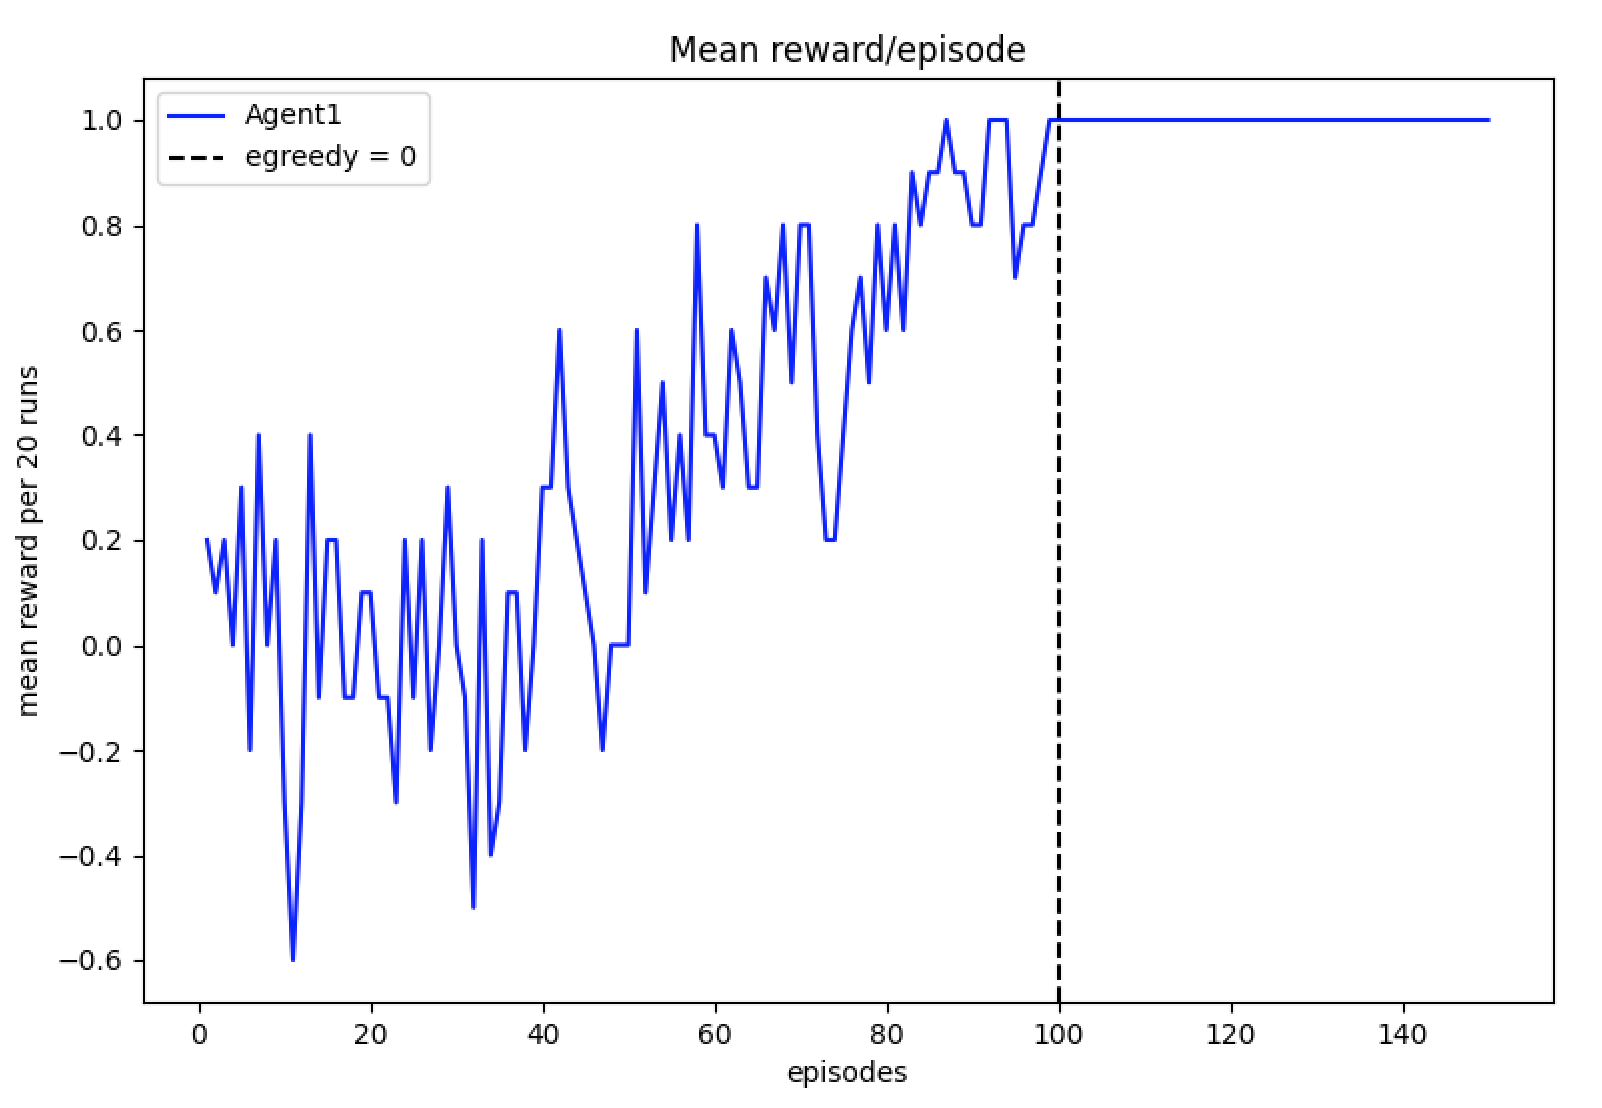
\includegraphics[width=80mm]{avg_reward_agent0}
		\caption{Average reward per episode for agent 1 \label{overflow}}
	\end{figure}
	
	
	\begin{figure}[ht!]
		\centering
		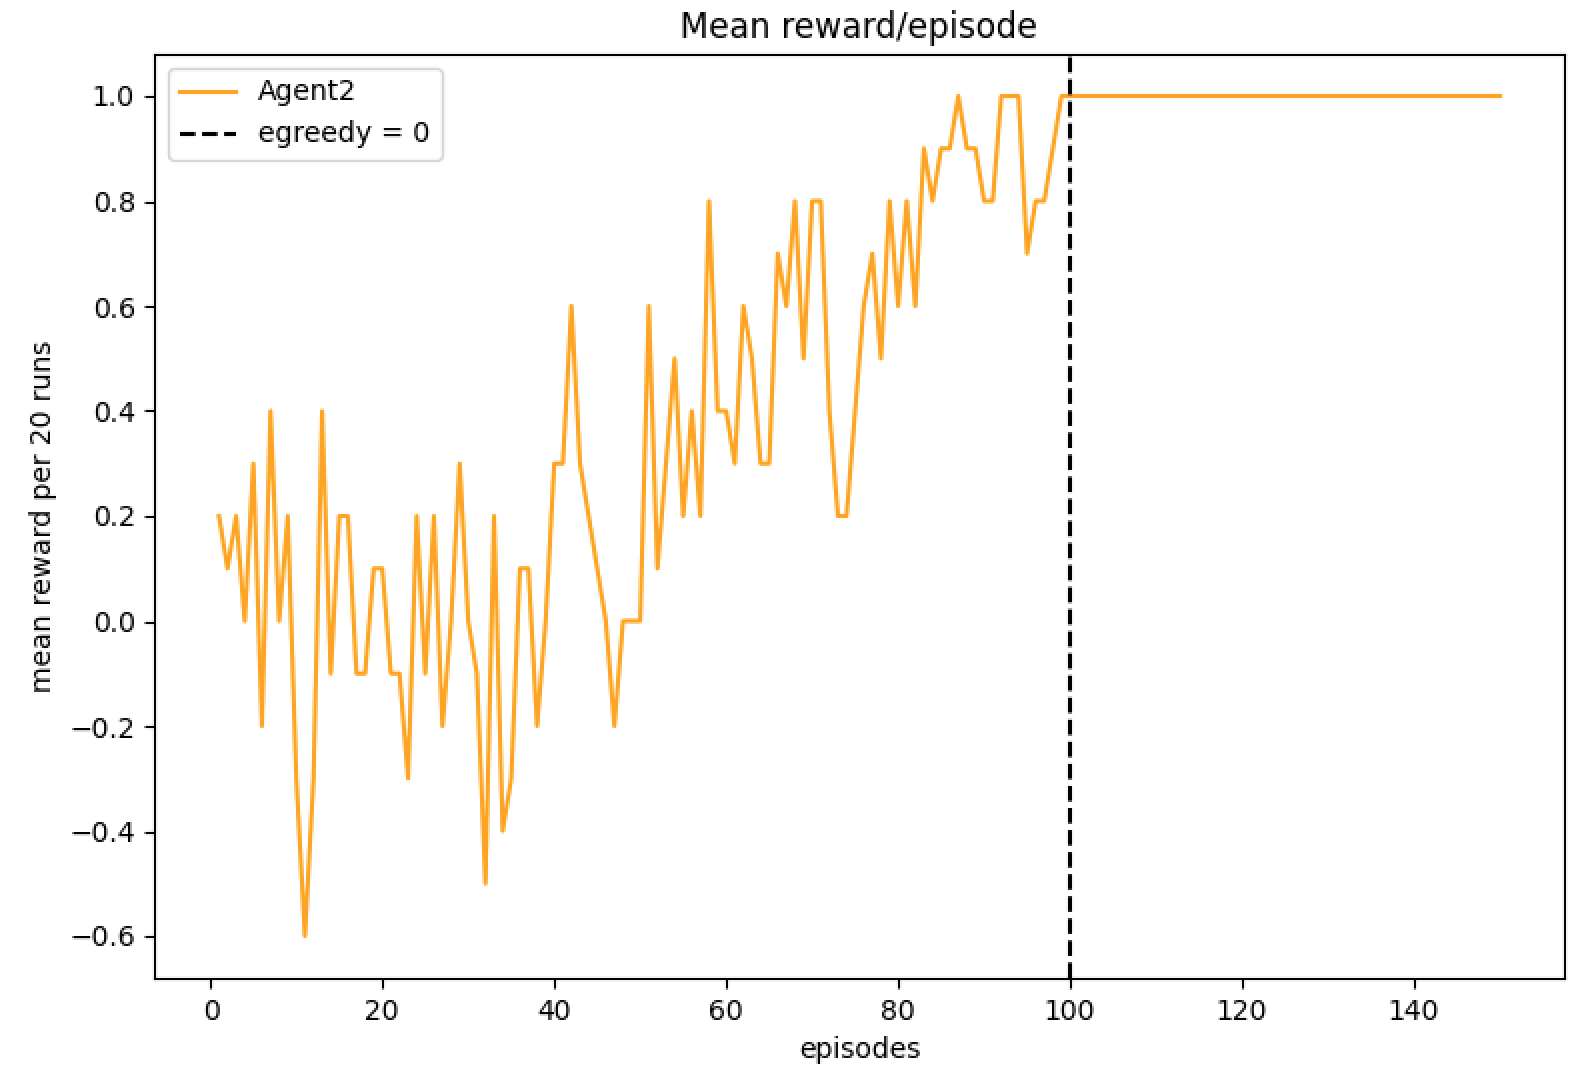
\includegraphics[width=80mm]{avg_reward_agent1}
		\caption{Average reward per episode for agent 2 \label{overflow}}
	\end{figure}
	
	Figures 1 and 2, depict the average reward both agents get at the completation of each episode. The vertical dashed line indicates that the exploration has stopped. As expected the agents receive the maximum possible reward after training which remains constant until the end of the remaining episodes.
	
	
	\begin{figure}[ht!]
		\centering
		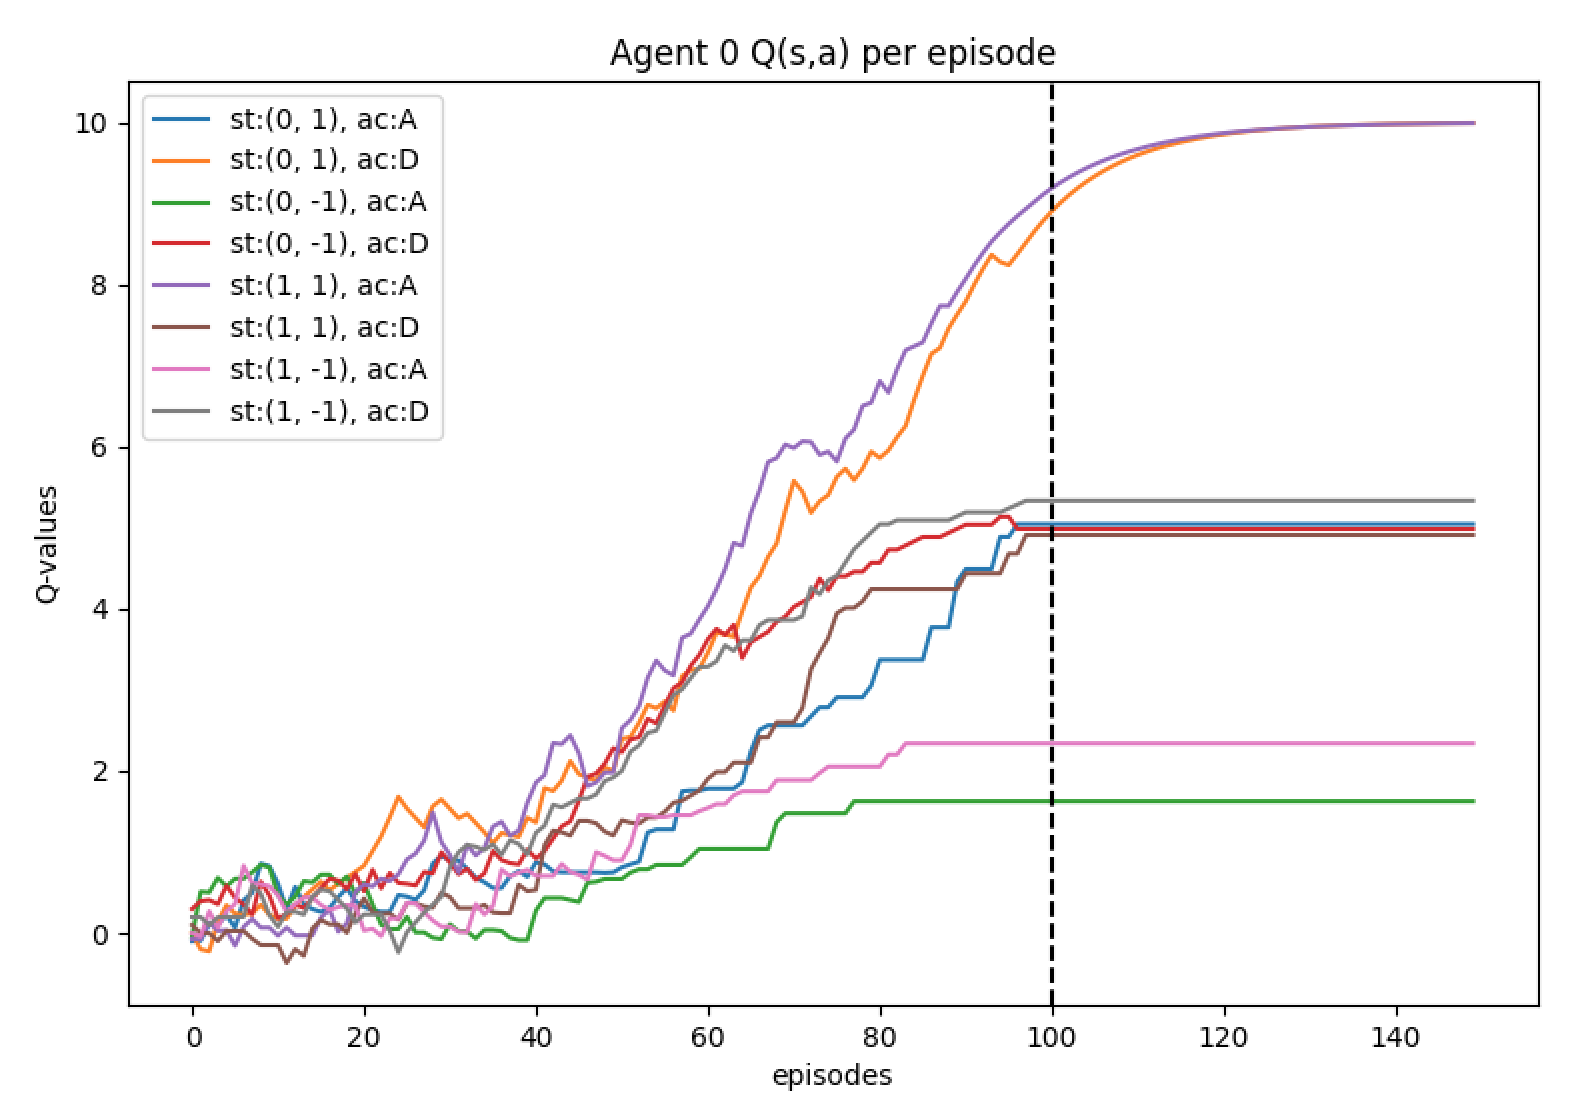
\includegraphics[width=80mm]{q_values_agent0}
		\caption{Q-values evolution per episode \label{overflow}}
	\end{figure}
	
	\begin{figure}[ht!]
		\centering
		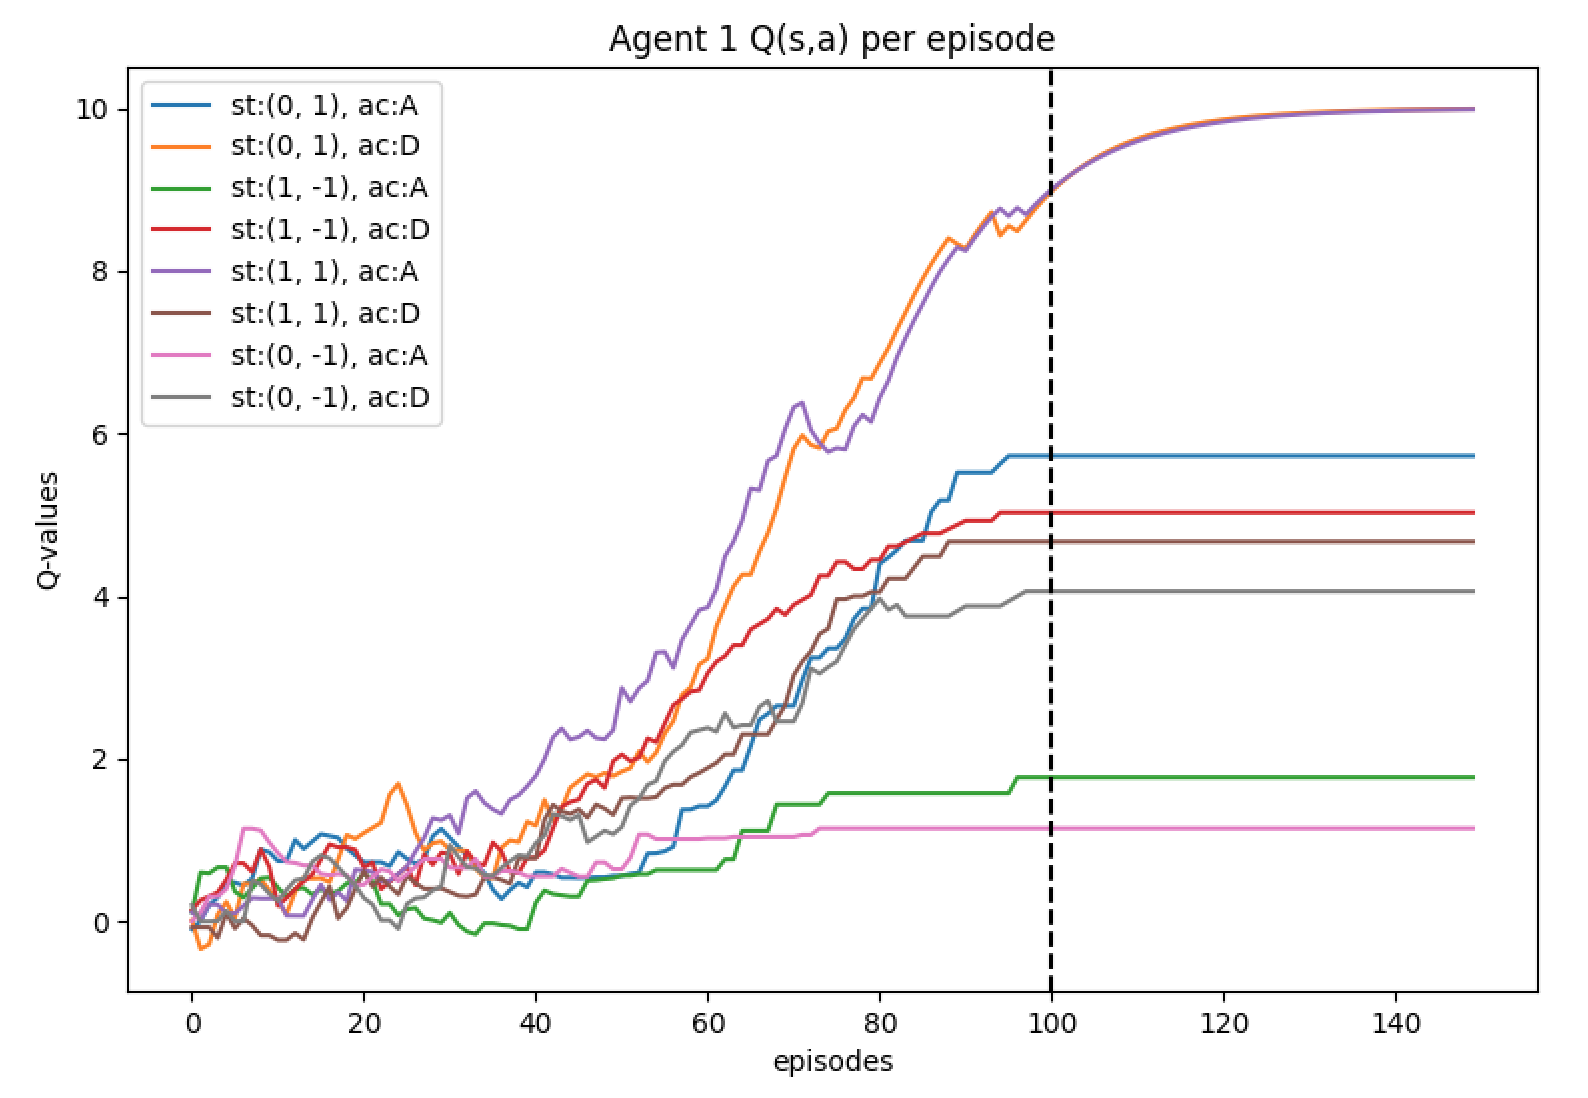
\includegraphics[width=80mm]{q_values_agent1}
		\caption{Q-values evolution per episode \label{overflow}}
	\end{figure}
	
	Next, we show the evolution of each discovered state/value combination for the 2 agents; figures 2 and 3. It is worth mentioning that our agents perceive the notion of a state as the tuple of (action,reward). Thus, Q-values are represented as Q(Action,Reward,Next-action). It seems the agents learned that 2 particular q-values would lead to maximization of total reward.
	
	Finally, we show the cumulative reward per agent during the whole simulation. Total time is defined as the product of \textit{number-of-episodes} times \textit{number-of-games}. At the time unit 2000, exploration stops and the reward increases linearly. This was hinted by figures 1 and 2. 
	
	As in Machine Learning in general, Reinforcement Learning has the so called \textit{hyper-parameters}. In this simulation we set the learning-rate $\alpha$ to 0.1 and the discount-factor $\gamma$ to 0.9 in order to make Q-values to converge. It is obvious the convergence depends also on the number of executed episodes. Lastly, it is possible for the two agents to reach Nash-Equilibrium \textbf{before} Q-values have converged.
	
	
	\begin{figure}[ht!]
		\centering
		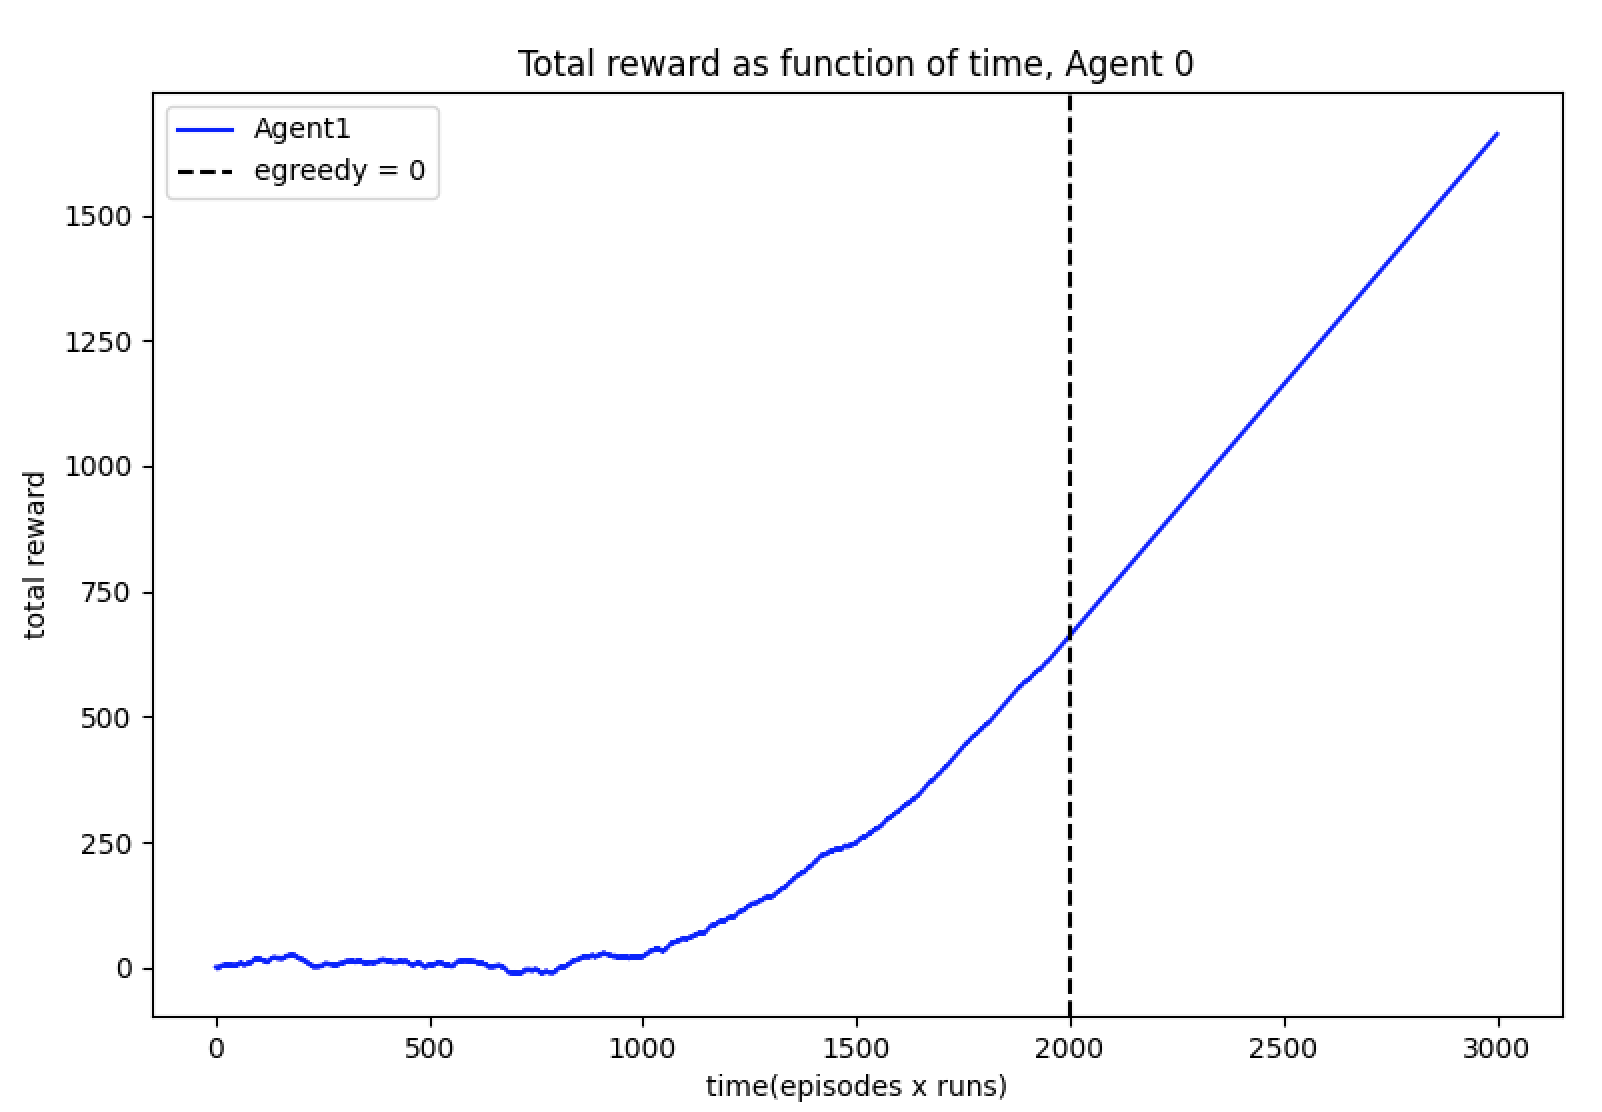
\includegraphics[width=80mm]{total_reward_agent0}
		\caption{Total reward agent 1 \label{overflow}}
	\end{figure}

	\begin{figure}[ht!]
	\centering
		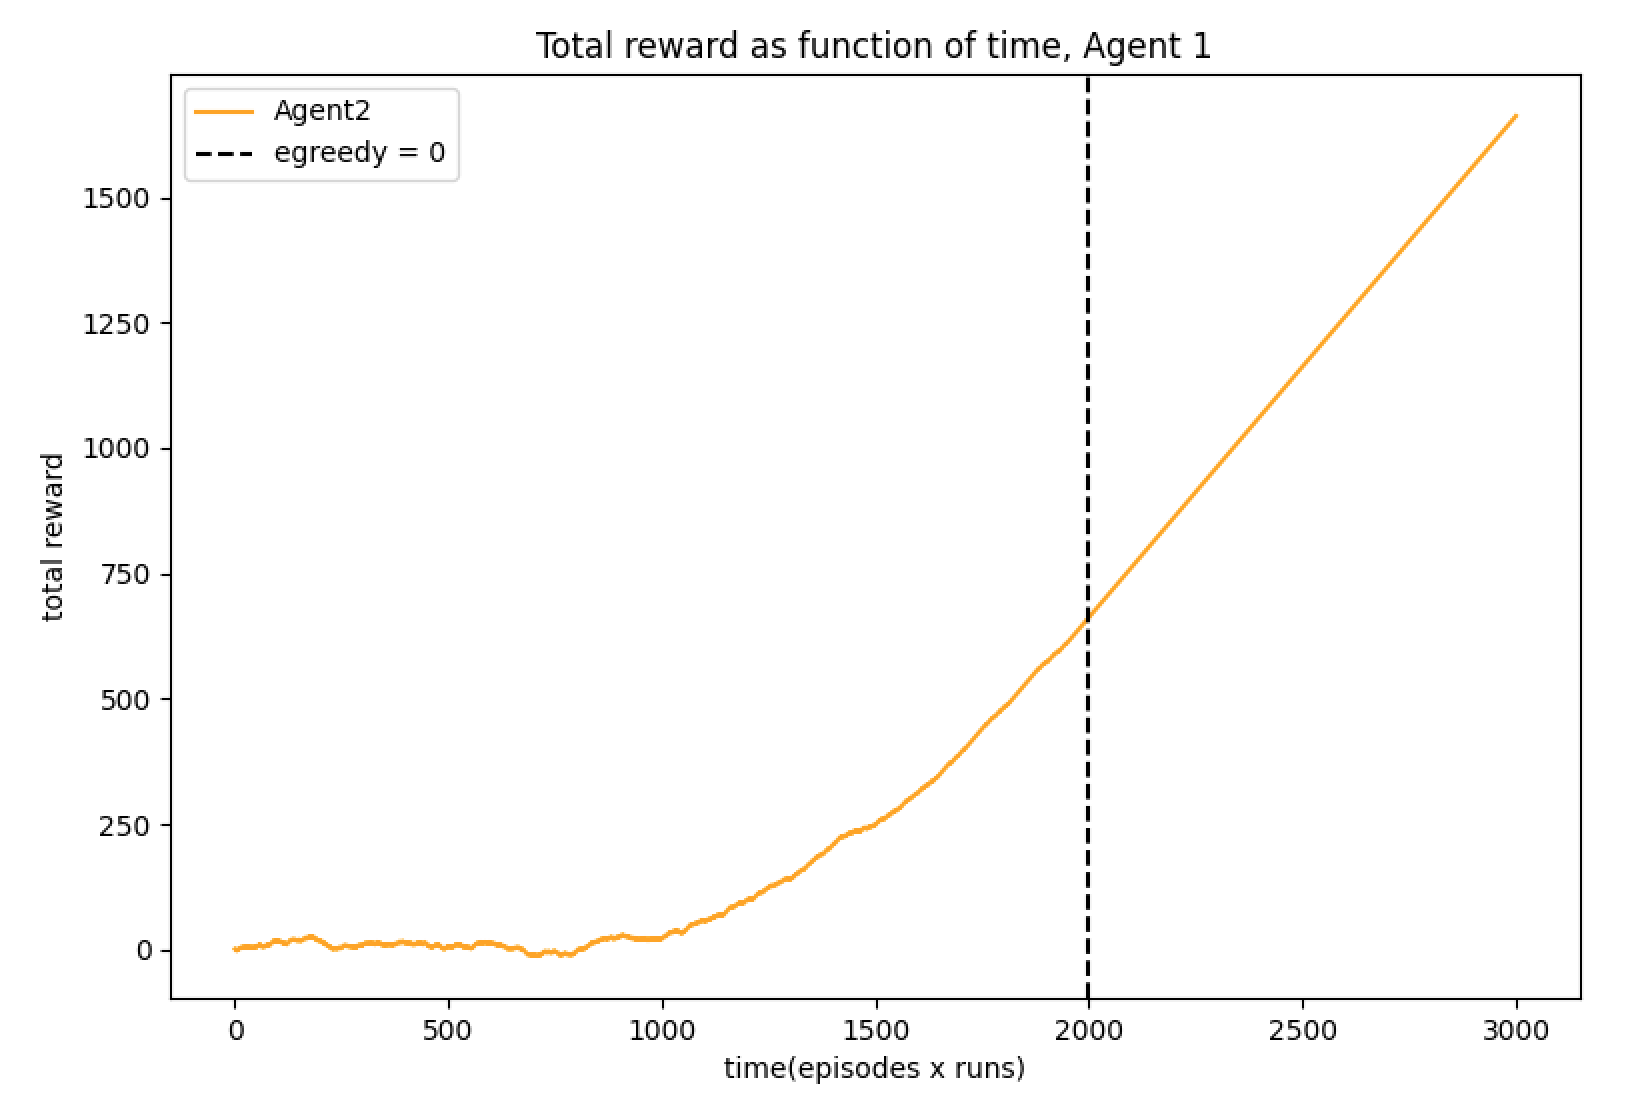
\includegraphics[width=80mm]{total_reward_agent1}
		\caption{Total reward agent 2 \label{overflow}}
	\end{figure}



	\section{Disclaimer}
	In order for our implemantion to be as generic as possible, we made the agents to \textit{discover} states. This means that we did not hard-coded the size of Q-table even though it was a trivial calculation. Furthermore, we tried other two approaches which led to similar results. One approach was to model the state space as the number of games(20 in this case) while the other one, since it is a stochastic game state space can be thought as a single state[3].	



	\begin{thebibliography}{9}
		\bibitem{russell} 
		Stuart Russell and Peter Norvig. 
		\textit{Artificial Intelligence: A Modern Approach}. 
		Prentice Hall, Fourth Edition 2020.
		
		\bibitem{sutton} 
		Sutton, R. and Barto, A. 
		\textit{Reinforcement Learning: An Introduction}. 
		MIT Press, 2017.
		
		\bibitem{wellman} 
		Junling Hu and Michael P. Wellman.
		\textit{Multiagent Reinforcement Learning: Theoretical Framework and an Algorithm}. 
		University of Michigan, Ann Arbor, MI 48109-2110, USA.

	\end{thebibliography}
	

\end{document}